\cotefile{126}
\scanpage{2}
% archive sheet number: 1

% slanted
\margin{Compléter, cf remarque 2 \uline{plus bas}}

\uline{Théorème} 1 \quad $f:X^{\unsure{\bullet|\circ|{}}}\longrightarrow S$ un morphisme \uline{\unsure{fid.} plat quasi-cpt}, \inserted{\uline{quasi-séparé}, \deleted{S} \uline{affine}} \inserted{\uline{couvrant quasi-compact quasi-séparé plat}}, $F$ faisceau quasi-cohérent sur $X$. Alors

\[
\unsure{H^i|\check H^i}(X^{\bullet}/S,F)\simeq
\begin{cases}0&\text{si }i\ne0\\ H^0(S,F)&\text{si }i=0\end{cases}
\]

On peut l'énoncer sous la forme suivante

\uline{Corollaire} 1 \quad \unsure{Hypothèse|Hypothèses} \unsure{précédente|précédentes}, sans hyp. affine sur $X$ cependant. Alors $\underline H^i(X^{\bullet}/S,F)$ (faisceaux \inserted{qu. coh.} sur $X$) \deleted{sont} \deleted{\unsure{isomorphes}} sont \unsure{nul|nuls} si $i\ne0$, et $F\longrightarrow\underline H^0(X\unsure{'|\bullet|^{\cdot}}/X,F)$ est un isomorphisme.

Or la formation \deleted{des} $\underline H^i(X^{\bullet}/S,F)$ est compatible avec extension \uline{plate} de \uline{la base}. [car les $X^{i}/S$ sont quasi-compacts quasi-séparés], et il suffit de prouver que les assertions dites sont vraies après changement de base plat couvrant $S_\lambda\longrightarrow S$, \inserted{les $S_\lambda$ affines.} Or on peut en trouver qui sont tels que les $X_\lambda/S_\lambda$ aient des sections, d'où le résultat, car pour $S$ affine et $X/S$ ayant une section, c'est immédiat.

% margin note written sideways
\margin{\uline{Corollaire} 2 Soit $X\longrightarrow S$ \uline{couvrant} \deleted{\unsure{q-comp.}} $H^0(S,F)\simeq \unsure{\check H^0|H^0}(X/S,F)$. Plus gén., le foncteur \deleted{à \unsure{tout} $S'$ \unsure{sur} $(Sch)/S$ qui associe} $S'\longmapsto\Gamma(S',F_{X_{S'}/S'})$ sur $(Sch)/S$ est un faisceau pour fpqc. En effet, on est ramené à le vérifier pour les deux types de familles couvrantes, Zariski, \unsure{et recouvrements|recouvrement} fid plats \deleted{\unsure{quasi-compacts}} \uuline{affines}}

\uline{Corollaire 3} Mettons sur $(Sch)$ une topologie $T$ intermédiaire entre celle de Zariski et la fpqc. Alors pour tt faisceau qu. coh. $F$ sur un $X$, $H^*_{\unsure{1|\,}}(X^T_{\unsure{T|\mathfrak{T}|1}},F^T)\simeq H^*(X,F)$

\uline{Dém} On est ramené par Leray pour $(Sch)^T\longrightarrow(Sch)^{\mathrm{Zar}}$, de prouver que pour \deleted{X} \uline{affine}, \unsure{-- --|on a}.
\scanpage{3}
% archive sheet number: 2

\[
H^{\unsure{i|j}}(X^T,F^T)=0,\quad H^0(X^T,F^T)\simeq H^0(X,F)
\]

\deleted{Pour} La \unsure{deuxième} relation triviale par définition de $F^T$.

Pour la première, \deleted{\unsure{on est}} (à prouver pour \uline{tt} \unsure{ouvert} affine) on est ramené par suite spectrale de Cartan : prouver que pour tt \deleted{\unsure{recouvrement} de $X$} famille couvrante $\unsure{\mathfrak X|\mathcal X}=(X_i\longrightarrow X)$, finie fid plate, $\check H^p(\mathfrak X,F)=0$ pour tt $p\ne0$.

\uline{Or} comme $F$ transforme sommes en produits, on peut supposer $\mathfrak X$ \unsure{réduit|réduite} à \uline{un} morphisme fid plat \deleted{\unsure{qu. cpct|quasi-compact}} de schémas affines. On est alors sous les conditions du Th. 1.

Utilisant la suite spectrale de Leray, on trouve

\uline{Corollaire 4} Soit $S'\longrightarrow S$ couvrant (pour la top. fpqc), $F$ qu. coh sur $S$. Alors on a une suite spectrale

\[
H^*(S,F)\Longleftarrow \check H^p(S'/S,{\unsure{\mathscr H|\mathcal H}}^q(F))
\]

[où $\mathscr H^q(F)$ désigne le foncteur $T\longmapsto H^q(T,F\otimes_S T)$ sur $(Sch)_{/S}^{\circ}$]
\scanpage{4}
% archive sheet number: 3

Notons \inserted{l'isomorphisme $H^0(S,F)\simeq H^0(S'/S,F)$ \uline{déjà connu}, et} la suite exacte en basses dimensions \unsure{et|d}

\[
0\longrightarrow\check H^1(S'/S,F)\longrightarrow H^1(S,F)\longrightarrow
\check H^0(S'/S,{\unsure{\mathscr H|\mathcal H}}^1(F))\longrightarrow
\check H^2(S'/S,F)\longrightarrow H^{\unsure{0|2}}(S,F).
\]

\uline{Remarques} 1) Bien entendu, on peut énoncer Cor. 4 également pour une \uline{famille} couvrante (fpqc.)

2) La démonstration du Th. 1 montre aussi, pour $S$ affine, que

\margin{?}

\[
\check H^p(S'/S,\mathscr H^q(F))=0 \qquad\text{pour \uline{tt} }p,\ \text{si }q\ne0
\]

\deleted{Ce résultat est sans doute \unsure{ne semble pas très|vrai semble peu|la suite spectrale} \unsure{intuitif|utilisé}.}

En particulier, on trouve

\[
\check H^0(S'/S,\mathscr H^q(F))=\operatorname{Ker}\bigl(H^q(S',F)\rightrightarrows H^q(S'\times_S S',F)\bigr)=0
\]

\deleted{Il en résulte en particulier,}

\figure{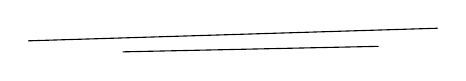
\begin{tikzpicture}\draw (0,0)--(5.2,.16);\draw (1.2,-.14)--(4.45,-.07);\end{tikzpicture}}

Application à l'effectivité des Relations d'équivalence :

\uline{Proposition} \quad $X$ un préschéma, $R$ une relation d'équivalence sur \unsure{$x$|$X$}, $X_0$ sous-préschéma de $X$ défini par un Idéal nilpotent, $X_0$ stable par $R$, $R_0$ la relation d'équivalence
\scanpage{5}
% archive sheet number: 4

induite sur $X_0$. On suppose que le \deleted{quotient $X_0/R_0$ \unsure{--}} $R_0$ est \unsure{(M)|(U)} effective, $M$ morphismes \deleted{\uline{couvrants} pour la top. fpqc}, et que \deleted{$R_0\overset{\unsure{p_i}}{\rightrightarrows}X_0$ soient} \inserted{et que $p_i^0:R_0\longrightarrow X_0$} \inserted{fid plats} qu. cpts, \deleted{\unsure{et}} qu. séparés.

Sous ces conditions, $R$ est \deleted{\unsure{(M)}} \inserted{M-} effective, \deleted{Et} \inserted{Si $X_0\longrightarrow Y_0$ est plate i.e. $R_0\longrightarrow X_0$}

\uline{Démonstration} \inserted{On peut supposer $\unsure{I|J|\mathcal J}_{X_0}$ de \uline{carré nul}.} Soit $Y_0=X_0/R_0$, alors $X_0\longrightarrow Y_0$ est couvrant, \deleted{\unsure{fid}} \uline{qu. cpct et qu. sép.} et $R_0\xrightarrow{\sim} X_0\times_{Y_0}X_0$.

Considérons $\underline I_{X_0},\underline I_{R_0}$, alors $\underline I_{X_0}$ est muni d'une \deleted{\unsure{relation}} donnée de \deleted{descente} \inserted{recollement} pour $X_0\longrightarrow Y_0$ \inserted{puis : $R_0\simeq X_0\times_{Y_0}X_0$,} [les deux images inverses \deleted{$I_{X_0}$} par $p^0_{10},p^0_{20}$ s'\deleted{\unsure{identifient}}\inserted{identifient} à $I_{X_0}$], c'est en fait une donnée de descente, comme elle \uline{est effective} \unsure{puis :|puisque :} $X_0\longrightarrow Y_0$ \uline{couvrant} et $R_0\simeq X_0\times_{Y_0} X_0$,
\scanpage{6}
% archive sheet number: 5

on trouve un $\underline{\unsure{I|J|\mathcal J}}_{Y_0}$ qu. coh. sur $Y_0$.

Pour prouver la M-effectivité de $R$, on peut supposer que $Y_0$ \deleted{\unsure{devient|descente} \unsure{$Y$|$X$}} affine. Soit alors $A_0$ l'anneau de $Y_0$, et \inserted{soit} \deleted{$A=\check H^0(X/\unsure{(X/R)|R}),\underline{\mathcal O}_X)$}

\[
A=\operatorname{Ker}\left(H^0(X,\mathcal O_X)\rightrightarrows H^0(R,\underline{\mathcal O}_R)\right)
\]

On a un hom évident $A\longrightarrow A_0$, dont le noyau est $\operatorname{Ker}\bigl(H^0(X_0,\underline I_{X_0})\rightrightarrows H^0(R_0,I_{R_0})\bigr)=H^0(Y_0,\underline I_{Y_0})=I_{Y_0}$. \deleted{\unsure{Il y a une suite}} \inserted{Je dis que la} \deleted{\unsure{suite ex}} suite d'hom

\[
0\longrightarrow I_{Y_0}\longrightarrow A\longrightarrow A_0\longrightarrow0
\]

est \uline{exacte}, i.e. $A\longrightarrow A_0$ \uline{surjectif}.

Pour le voir, \deleted{prenons} soit $\varphi_0\in A_0$, soit $f_0$ son image \inserted{inverse} dans $X_0$, \deleted{$f_0\in H^0(X_0,\mathcal O_{X_0})$} \inserted{donc}

\[
f_0\in\operatorname{Ker}\left(H^0(X_0,\mathcal O_{X_0})\rightrightarrows H^0(R_0,\mathcal O_{R_0})\right)
\]

Je dis d'abord que $f_0$ se remonte en un $f\in H^0(X,\underline{\mathcal O}_X)$. En effet, à priori il y a une obstruction à relever qui est \deleted{dans} $\unsure{\zeta|\xi}\in H^1(X_0,I_{X_0})$ ; mais les deux images
\scanpage{7}
% archive sheet number: 6

inverses de \deleted{cette} \unsure{dernière|dernier}, par $p_1^0$ \unsure{ou|et} $p_2^0$, sont identiques, car ce sont les obstructions à relever une $=$ section $g_0\in H^0(R_0,\mathcal O_{R_0})$ en un $g\in H^0(R,\mathcal O_R)$. D'où

\[
\begin{aligned}
\unsure{\zeta|\xi}&\in\operatorname{Ker}\bigl(H^1(X_0,\unsure{I|J|\mathcal J}_{X_0})\rightrightarrows H^1(R_0,I_{R_0})\bigr)\\
&=\check H^0(X_0/Y_0,{\unsure{\mathscr H|\mathcal H}}^1(\underline I_{Y_0}))
\end{aligned}
\]

or on sait que le $2^{\mathrm{ième}}$ mb est nul, $X_0\longrightarrow Y_0$ étant couvrant qu. cpct et qu. séparé. Par suite on trouve $\zeta=0$, d'où l'existence d'un $f$. Si on avait \deleted{$f\in\operatorname{Ker}$} $p_1(f)=p_2(f)$,

on aurait gagné, car $f$ proviendrait d'un $\varphi\in A$, qui \deleted{\unsure{redonnerait} \unsure{par}} \inserted{relèverait} donc $\varphi_0$.

\diagram{\begin{tikzcd}[ampersand replacement=\&,column sep=small,row sep=small]
\& f \& {}\\
A\arrow[r]\arrow[d] \& H^0(X,\underline{\mathcal O}_X)\arrow[r,shift left=.6ex,"p_1"]\arrow[r,shift right=.6ex,"p_2"']\arrow[d] \& H^0(R,\mathcal O_R)\arrow[d]\\
A_0\arrow[r] \& H^0(X_0,\mathcal O_{X_0})\arrow[r,shift left=.6ex]\arrow[r,shift right=.6ex] \& H^0(R_0,\mathcal O_{R_0})\\
\varphi_0\& f_0\&{}
\end{tikzcd}}

À priori, on peut seulement dire que $y\unsure{\in|=}p_1(f)-p_2(f)\in H^0(R_0,I_{R_0})$ d'ailleurs on vérifie que

\[
y\in{\unsure{\mathbb Z|Z}}^{1}(X_0/Y_0,\underline I_{Y_0})\qquad\text{i.e. }dy=0
\]

D'ailleurs, on dispose de l'arbitraire de $\lambda\in H^0(X_0,\underline I_{X_0})$ pour $f$, et on voit que \deleted{la correction} dire que $p_1(f+\lambda)=p_{\unsure{2|\,}}(f+\lambda)$ signifie que $p_2(\lambda)-p_1(\lambda)=\deleted{\unsure{u|\text{«}}}y$, i.e.

\[
d(\lambda)=y.
\]
\scanpage{8}
% archive sheet number: 7

On sait que ($X_0\longrightarrow Y_0$ \unsure{étant} couvrt qu. cpct qu. sép.)

\[
\check H^1(X_0/Y_0,\underline{\unsure{I|J|\mathcal J}}_{Y_0})=0
\]

donc on peut résoudre l'équation $d(\lambda)=y$, ce qui prouve la surjectivité annoncée.

\deleted{Soit} Soit $Y=\operatorname{Spec} A$, alors \deleted{$A$} on obtient un diagramme commutatif

\diagram{\begin{tikzcd}[ampersand replacement=\&]
Y\&X\arrow[l]\&R\arrow[l,shift left=.8ex]\arrow[l,shift right=.8ex]\\
Y_0\arrow[u,<->]\&X_0\arrow[l]\arrow[u]\&R_0\arrow[l,shift left=.8ex]\arrow[l,shift right=.8ex]\arrow[u]
\end{tikzcd}}

D'ailleurs, \deleted{\unsure{posons|pour} $\underline I_{Y_0}$} par l'exactitude écrite précédemment, $Y_0$ est un sous-schéma fermé de $Y$ défini par un idéal nilpotent isomorphe à $\underline I_{Y_0}$.

On voit de suite que

\[
\underline I_{Y_0}X=\underline I_{X_0}\simeq\underline I_{Y_0}\unsure{\otimes_{Y_0}|\mathcal O_{Y_0}|\otimes_{\mathcal O_{Y_0}}}\mathcal O_{X_0}
\]

comme Idéal sur $X$, i.e. $X_0\longrightarrow Y_0$ déduit de $X\longrightarrow Y$ par changement de base $Y_0\longrightarrow Y$. Comme de plus $X_0/Y_0$ est plat, $X/Y$ est \uline{plat}. Comme $R\longrightarrow X$ est plat, $R$ est plat sur $Y$, et $R\longrightarrow X\times_Y X=P$ est un morphisme de $Y$-préschémas \uline{plats}, tels que $R_0\longrightarrow P_0$ est un isom, donc $R\longrightarrow P$ est un isomorphisme, O.K.
\scanpage{9}
Généralités sur la topologie fpqc

les $\check H^p(S'/S,{\unsure{\mathscr H|\mathcal H}}^q(F))$ pour $F$ quasi-cohérent.

Application aux relations d'équivalence .....

% archive sheet number: 8
\scanpage{10}
\uline{Proposition 1} \quad $C$ catégorie \inserted{avec \deleted{\unsure{les}} produits fibrés} munie d'une prétopologie $T$, \deleted{\unsure{et}} $C'$ \deleted{$\subset\operatorname{Ob}C$} \inserted{sous-catégorie \deleted{stable} pleine de $C$} \deleted{système de} \uline{\unsure{génératrice|générateurs}} pour $T$ \deleted{stable par isomorphisme et produits fibrés}

\textcircled{a} pour tt $X\in\operatorname{Ob}C$, existe famille couvrante $U_\alpha\longrightarrow X$ pour $T$, avec les $U_\alpha\in\operatorname{Ob} C'$], \deleted{\unsure{tt}}

\textcircled{b} $C'$ stable par isomorphie et produits fibrés, \deleted{\unsure{et}}

\deleted{et de flèches pour la} $T'$ une \deleted{prétopologie sur de flèches de la catégorie de $C$} \inserted{prétopologie sur $C'$. On suppose} \deleted{\unsure{formée}}

\textcircled{c} \deleted{$T'$ stable par composition, par changement de base, et admet les \deleted{identités} isomorphismes entre objets de $C'$.}

\deleted{Soit $\unsure{\mathfrak T|\mathcal T|\mathcal C}$ la topologie engendrée par $T,T'$. Soit $X_i\longrightarrow X$ une famille de flèches. Pour qu'elle soit couvrante pour $T$, il f. et s. \unsure{que pour des}}

que dans la situation

\diagram{\begin{tikzcd}[ampersand replacement=\&,row sep=small,column sep=small]
\& U_{ij\unsure{h|k|\mu}}\arrow[d]\\
\deleted{\unsure{X}}U_i\arrow[d] \& U_{ij}\arrow[l]\\
U \& {}
\end{tikzcd}}

où $U,U_i,U_{\unsure{ij|j}},U_{ijh}\in\operatorname{Ob} C'$, $(U_i\longrightarrow U)$ et $(U_{ijh}\longrightarrow U_{ij})$ couvrant pour \deleted{\unsure{la}} $T'$, et $(U_{ij})\longrightarrow U_i$ couvrant pour $T$, on peut trouver une sous-famille des $U_{ijh}\longrightarrow U$ couvrante pour $T'$.

% archive sheet number: 9
\scanpage{11}
Soit $\unsure{\mathscr T|\mathcal T}$ la topologie engendrée par $T,T'$, \deleted{Pour} et soit $X_i\longrightarrow X$ une famille de morphismes de $C$. Pour qu'elle soit $\mathscr T$-couvrante, il f et s qu'il existe une famille $T$-couvrante $U_\alpha\longrightarrow X$, \inserted{$U_\alpha\in\operatorname{Ob}C'$,} et pour tt $\alpha$ une

\diagram{\begin{tikzcd}[ampersand replacement=\&]
X_i\arrow[d] \& U_{\alpha\beta}\arrow[l]\arrow[d]\\
X \& U_\alpha\arrow[l]
\end{tikzcd}}

famille $T'$-couvrante $U_{\alpha\beta}\longrightarrow U_\alpha$, et pour tt $\beta$ un indice $i$ et un $X$-morphisme $U_{\alpha\beta}\longrightarrow X_i$.

\inserted{\uuline{Cor} 1} Si $X=\deleted{U}{\unsure{X|U|{}}}\in\operatorname{Ob}C'$, il f. et s. aussi qu'il existe $U_\alpha\longrightarrow\deleted{\unsure{U}}X$ \uline{couvrant pour $T'$}, \deleted{que} et pour tt $\alpha$ un $i$ \deleted{tel que} et un $X$-morphisme $U_\alpha\longrightarrow X_i$.

% slanted
\margin{N.B. le complément résulte de la proposition, grâce à condition \textcircled{c}}

\uline{Dém} Si cette condition est remplie, alors $U_{\alpha\beta}\longrightarrow X$ est couvrante pour $\mathscr T$ par transitivité, et par suite $X_i\longrightarrow X$ l'est par saturation. Il reste à prouver que les familles du type envisagé satisfont les conditions 1) 2) 3) 4). Pour 4) c'est trivial,

\deleted{pour} 3) aussi [\inserted{si $X'\xrightarrow{\sim}X$,} prendre une famille couvrante $\deleted{\unsure{X|U}}U_\alpha$ de $X$ par des $U_\alpha\in\operatorname{Ob}C'$ -- existe par hypothèse \inserted{\textcircled{a}} \deleted{que $C'$ génératrice de $(C,T)$}, $(U_{\alpha\beta})_\beta$ réduit à $U_\alpha$ \unsure{---} $U_\alpha\xrightarrow{\mathrm{id}}U_\alpha$, et $U_\alpha\longrightarrow X'$ déduit de $U_\alpha\longrightarrow X$. Pour \unsure{2)|1)},

% archive sheet number: 10
\scanpage{12}
\deleted{Alors} Pour tt $\alpha$, il existe par construction $i$\deleted{\unsure{ puis}} $j$ \deleted{tels} et un $X$-morphisme $\deleted{U_{\alpha\unsure{\beta\gamma\delta|\beta\delta|\beta}}\longrightarrow} V_{\alpha\lambda}\longrightarrow X_{ij}$, OK.

\uuline{Cor. 2} Soit $F:\deleted{\unsure{(Sch)}}C^{\circ}\longrightarrow(Ens)$, pour que $F$ soit un faisceau \inserted{pour $\unsure{\mathscr T|\mathcal T}$}, il f. et s que $F$ \deleted{\unsure{satisf. induise un}} \inserted{en soit un} pour $T$, et \deleted{pour t} induise sur $C'$ un faisceau pour $T'$.

% slanted
\margin{\deleted{\unsure{Évid.}} En effet, nécessité triviale, pour la suffisance on note que l'ens. des familles qui \deleted{\unsure{satisf.}} \inserted{sont des} $F$-\unsure{descentes} forme une \uline{topologie}, qui \unsure{comprend|en prend|pour} $T,T'$ donc $\mathscr T$, OK}

\uline{Proposition} 2 Considérons sur $(Sch)=C$ la prétopologie $T$ de Zariski. Considérons de plus sur la sous-catégorie pleine $C'$ de $C$ formée des \unsure{ouverts|schémas} affines la prétopologie suivante :

% slanted
\margin{\uline{Ex} Cat $(Sch)$ fpqc : Zariski-\unsure{fin|fam|topologie} : un $f:U\longrightarrow V$ fid plat, $U,V$ affines}

% slanted
\margin{\unsure{resp} plate aussi plate de présentation finie, plate de prés. finie et quasi-finie, étale,}

une famille \deleted{$\longrightarrow$} $U_i\longrightarrow U$ est couvrante, si elle est finie, \deleted{et fid} \inserted{surjective et} plate [i.e. les $U_i$ sont en nb fini, les images recouvrent $U$, et les $U_i\longrightarrow U$ sont plats]. Soit $\mathscr T$ la topologie \inserted{sur $C$} engendrée par $T,T'$.

(i) Soit $X_i\longrightarrow X$ une famille de morphismes dans $C$. Pour qu'elle soit couvrante, il f. et s. que \deleted{\unsure{q.}} $X$ puisse se recouvrir par des ouverts affines $U_\alpha$ et que pour tt $\alpha$ $\exists$ une famille finie fid plate $U_{\alpha\beta}\longrightarrow U_\alpha$, les $U_{\alpha\beta}$ affines, \deleted{telle que} et pour tt $\alpha,\beta$ un $i=i(\alpha,\beta)$ et un $X$-morphisme $U_{\alpha\beta}\longrightarrow \unsure{X|X_i}$.

\diagram{\begin{tikzcd}[ampersand replacement=\&]
X_i\arrow[d,dash] \& U_{\alpha\beta}\arrow[l]\arrow[d]\\
X\&U_\alpha\arrow[l]
\end{tikzcd}}

% archive sheet number: 11
\scanpage{13}
% The return arrow moves (ii), including a), b) and the display, before (iii).
\inserted{\deleted{\unsure{(iii)}} (ii) Soit $F:(Sch)^{\circ}_{\unsure{/S|S|{}}}\longrightarrow(Ens)$ un foncteur. Pour que $F$ soit un faisceau pour $T$, il f. et s. qu'il satisfasse les conditions suivantes}

a) $F$ est un faisceau pour la topologie de Zariski i.e. \deleted{b)} ``$F$ de nature locale''

b) Pour tt $S'\longrightarrow S$ fid plat, avec $S$ et $S'$ affines, on a exactitude dans

\[
F(S)\longrightarrow F(S')\rightrightarrows F(S'\times_S S^{\unsure{\prime|\circ}})
\]

(iii) Un morphisme fid plat quasi-compact $f:X'\longrightarrow\deleted{S}X$ est couvrant pour $\unsure{\mathscr T|\mathcal T}$. De $=$ un morphisme fid plat \deleted{loc de présentation fi} \inserted{ouvert, p. ex.} un morphisme fid plat loc. de prés. finie ; Plus généralement, si on a une famille de morphismes $X_i\longrightarrow X$ \uline{ouverts}, \uline{plats}, dont les images recouvrent $X$, cette famille recouvre $X$ pour $\mathscr T$.

\uline{Dém} (i) résulte de Prop 1.

(ii) Nécessité triviale, pour la suffisance, on \deleted{peut \unsure{facilement montrer} que $F$ \unsure{convient}} \inserted{applique Cor. 1 sur \unsure{Théorème|Théorèm|corollaire} 2., \uline{en notant}} \deleted{pour les morphismes fid plats et qu. cpcts [étant donné que ceux-ci sont stables par}

% archive sheet number: 12
\scanpage{14}
\diagram{\begin{tikzcd}[ampersand replacement=\&,row sep=small,column sep=small]
X_i\arrow[d] \& U_{\alpha\beta}\arrow[l]\arrow[d] \& {} \& {}\\
X\&U_\alpha\arrow[l] \& {} \& {}\\
{}\&X'_i\arrow[d]\arrow[uul] \&U'_{\alpha\beta}\arrow[l]\arrow[d]\arrow[uul] \& U'_{\alpha\beta\lambda}\arrow[l]\arrow[d]\\
{}\&X'\arrow[uul]\&U'_\alpha\arrow[l]\arrow[uul]\&U'_{\alpha\lambda}\arrow[l]
\end{tikzcd}}

on note que les $U'_\alpha$ recouvrent $X'$ pour $T$ ; \deleted{\unsure{et}} pour tt $\alpha$, recouvrons \inserted{pour $T$} $U'_\alpha$ par des $U'_{\alpha\lambda}\in\operatorname{Ob}C'$, (possible par hyp \textcircled{\unsure{a|b}}), d'où des $U'_{\alpha\beta\lambda}$, pour $\alpha$ et $\lambda$ fixés, les $U'_{\alpha\beta\lambda}$ recouvrent $U'_{\alpha\beta}$ pour $T'$ ; \inserted{grâce à \textcircled{b}, car déduits de $U_{\alpha\beta}\longrightarrow U_\alpha$ par changt de base,} de plus pour $\alpha,\lambda$ variables, les $U'_{\alpha\lambda}$ recouvrent $X'$ pour $T'$, par transitivité OK.

Axiome \unsure{1|2} de transitivité, On construit

\diagram{\begin{tikzcd}[ampersand replacement=\&,row sep=small,column sep=small]
\unsure{V_{ij}|X_{ij}}\arrow[d,dash] \& X_{\unsure{j|ij}}\times_{X_i}U_{\alpha\beta}\arrow[l]\arrow[d] \& U_{\alpha\beta\gamma\delta}\arrow[l]\arrow[d]\\
X_i\arrow[d] \& U_{\alpha\beta}\arrow[l]\arrow[d] \& U_{\alpha\beta\gamma}\arrow[l]\\
X \& |[draw,circle,inner sep=1pt]|U_\alpha\arrow[l]\&{}
\end{tikzcd}}

grâce à l'hyp. \inserted{sur} $X_i\longrightarrow X$ \deleted{couvrant} des $U_\alpha,U_{\alpha\beta}$, et pour tout $\alpha,\beta$ un $U_{\alpha\beta}\longrightarrow X_i$, \inserted{$i=i(\alpha,\beta)$,} alors par le point \unsure{vient|qu'on vient} de voir, la famille des $X_{ij}\times_{X_i} U_{\alpha\beta}$ ($j$ variable) satisfait aux conditions envisagées, donc $\exists$ $U_{\alpha\beta\gamma}\longrightarrow U_{\alpha\beta}$ couvrant pour $T$, les $U_{\alpha\beta\gamma}\in\operatorname{Ob}C'$, et \deleted{pour} tt $\gamma$ une famille $U_{\alpha\beta\gamma\delta}\longrightarrow U_{\alpha\beta\gamma}$ couvrante pour $T'$, et un $j=j(\gamma,\delta)$ et $U_{\alpha\beta}$-morphisme $U_{\alpha\beta\gamma\delta}\longrightarrow \deleted{\unsure{U|X}}X_{ij}\times_{X_i}U_{\alpha\beta}$. Par \textcircled{c}, on peut pour tt $\alpha$, extraire des $U_{\alpha\beta\gamma\delta}\longrightarrow U_\alpha$ une famille couvrante pour $T'$, soit $V_{\alpha\lambda}\longrightarrow U_\alpha$.

% archive sheet number: 13
\scanpage{15}
\deleted{changement de base \uline{dans $C$}, et engendrent $\unsure{\mathscr T|\mathcal T}$ avec la prétopologie de Zariski). Or pour ceci, il suffit de}

\diagram{\begin{tikzcd}[ampersand replacement=\&]
S'\arrow[d]\&{}\\
S\&S_\alpha\arrow[l]
\end{tikzcd}}

que grâce à condition a), $F$ \deleted{\unsure{commute}} transforme déjà sommes en produits, ce qui pour vérifier la condition \unsure{2°|2)|b)} du corollaire 1, nous permet de nous ramener au cas d'un seul morphisme.

\deleted{\unsure{(ii)}} \inserted{(iii)} pas de problèmes.....

% archive sheet number: 14
\scanpage{16}
\uline{Descente fidèlement plate}

% archive sheet number: 15
\scanpage{18}
\deleted{\unsure{1|2}} A) Application à la comparaison avec les revêtements étales holomorphes

B) Application à \deleted{la construction} \inserted{une factorisation} canonique

\uline{Proposition} \quad Soit $f:X\longrightarrow Y$ un morphisme fini, \inserted{\uuline{univ. ouvert}}, \deleted{\unsure{sur}} avec $Y$ loc noethérien. \deleted{\unsure{Supposons|Pour}} \inserted{Pour} $y\in Y$, soit $d(y)$ le nb de pts géométriques de $f^{-1}(y)$ ($=$ degré séparable de $f^{-1}(y)$ sur $k(y)$]

\uline{Supposons} $d(y)$ \unsure{loc. cste.|constant} Alors $f$ se factorise en $X\xrightarrow{f_1}X'_0\xrightarrow{f_2}Y$ où $f_1$ est \inserted{fini,} surjectif radiciel, et $f_2$ est un morphisme \uline{fini} \uline{étale}. \inserted{\uline{Alors}} \uline{Tout} $Y$-morphisme $X\longrightarrow Z$, \margin{\unsure{1}} avec $Z$ étale sur $Y$, se factorise de façon unique en $X\longrightarrow X'\longrightarrow Z$.

On peut supposer \inserted{$Y$ connexe donc} $d(y)$ constant, soit $n$. (quitte à remplacer $Y$ par une partie à la fois ouverte et fermée convenable, pour \unsure{tt entier|la notion}]

% Mirrored printing shows through from the other face of the sheet.

% archive sheet number: 17
